\documentclass[twoside]{article}
\usepackage[a4paper]{geometry}
\geometry{verbose,tmargin=2.5cm,bmargin=2cm,lmargin=2cm,rmargin=2cm}
\usepackage{fancyhdr}
\pagestyle{fancy}

% nastavení pisma a~češtiny
\usepackage{lmodern}
\usepackage[T1]{fontenc}
\usepackage[utf8]{inputenc}
\usepackage[czech]{babel}

% odkazy
\usepackage{url}

\usepackage{float}
% vícesloupcové tabulky
\usepackage{multirow}
\usepackage{amssymb}
\usepackage{gensymb}
\usepackage{bbold}
\usepackage{amsmath}
\usepackage{mathtools}
\usepackage{commath}

% vnořené popisky obrázků
\usepackage{subcaption}

% automatická konverze EPS 
\usepackage{graphicx} 
\usepackage{epstopdf}
\epstopdfsetup{update}

\graphicspath{{./images}}

% odkazy a~záložky
\usepackage[unicode=true, bookmarks=true,bookmarksnumbered=true,
bookmarksopen=false, breaklinks=false,pdfborder={0 0 0},
pdfpagemode=UseNone,backref=false,colorlinks=true] {hyperref}

% Poznámky při překladu
\usepackage{xkeyval}	% Inline todonotes
\usepackage[textsize = footnotesize]{todonotes}
\presetkeys{todonotes}{inline}{}

%https://tex.stackexchange.com/questions/2783/bold-calligraphic-typeface
\DeclareMathAlphabet\mathbfcal{OMS}{cmsy}{b}{n}

% Zacni sekci slovem ukol
\renewcommand{\thesection}{Úkol \arabic{section}}
% enumerate zacina s pismenem
\renewcommand{\theenumi}{\alph{enumi}}

% smaz aktualni page layout
\fancyhf{}
% zahlavi
\usepackage{titling}
\fancyhf[HC]{\thetitle}
\fancyhf[HLE,HRO]{\theauthor}
\fancyhf[HRE,HLO]{\today}
 %zapati
\fancyhf[FLE,FRO]{\thepage}

% údaje o autorovi
\title{Automatické řízení: DÚ 7 -- Frekvenční metody}
\author{Vojtěch Michal}
\date{\today}

\begin{document}

\maketitle

\section{Nastavení zesílení regulátoru na požadovaný překmit}
Uvažujte soustavu s přenosem otevřené smyčky
\begin{equation}
	L(s) = \frac{K}{s(s+50)(s+100)}
\end{equation}
a) použijte frekvenční metody k návrhu zesílení $K$ tak, aby měl výsledný zpětnovazební systém
(uzavřená smyčka) překmit na skok reference 20\%. \\
b) Výsledek ověřte simulací. \\
\textbf{Řešení:}
Zadaný maximální překmit nám určuje minimální damping ratio
\begin{equation}
	\zeta = \frac{-\ln(\text{\%OS}/100)}{\sqrt{\pi^2 + \ln^2(\text{\%OS}/100)}} = 0.45595,
\end{equation}
které lze převést na požadovanou fázovou jistotu (\textit{phase margin})
\begin{equation}
	\text{PM} = \text{arctg} \left( \frac{ 2 \zeta}{-2\zeta^2 + \sqrt{1 + 4 \zeta^4}} \right) = 0.8403~\text{rad} = 48.148~\deg.
\end{equation}

Vykresleme Bodeho frekvenční charakteristiku pro open loop přenos $L(s)$, kde zatím neznámé zesílení regulátoru $K$
nahradíme jedničkou. Charakteristika je na obrázku \ref{fig:bode_unity_gain}.

\begin{figure}[htbp]
	\centering
	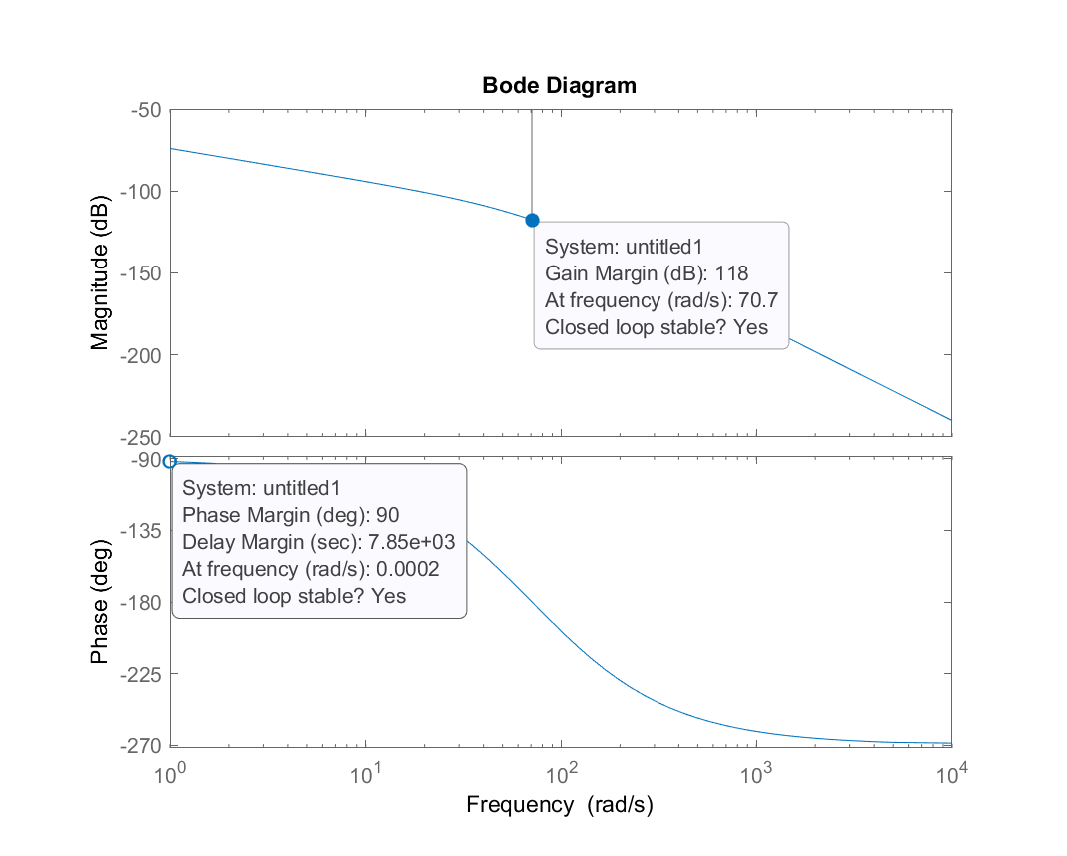
\includegraphics[width=0.65\linewidth]{bode_unity_gain.eps}
	\caption{Bodeho char. $L(s)$ pro $K=1$}
	\label{fig:bode_unity_gain}
\end{figure}


Tento výsledek je očekávatelný. Otevřená smyčka je kompletně bez nul a zbylé dva póly má výrazně dále
vlevo než jeden dominantní pól v počátku. Díky tomu je pro nízké frekvence konstatní fáze -90° a
klesá až od cca 5 rad/s, protože druhý nejbližší pól je na frekvenci 50 rad/s.
Je tak očekávatelné, že se na fázový posun -180° dostaneme až na relativně velké frekvenci,
kdy již bude modul zatlumený, neboť bez regulátoru je přechodová frekvence pouhých 0.0002 rad/s.

Regulátor proto musí velmi výrazně zvednout zesílení otevřené smyčky,
aby se uzavřená smyčka chovala podle požadavků. 
Potřebujeme phase margin vypočtený výše, takže na \textit{gain crossover frequency} $\omega_c$
musí být fáze open loop přenosu rovna $\varphi = -180\degree + \text{PM} = -131.852\degree$. Odečtením z 
amplitudové char. na obrázku \ref{fig:bode_crossover} zjistíme, že dané fáze je nabýváno na nové přechodové 
frekvenci $\omega_c \approx 25$ rad/s.
Modul openloop přenosu je tehdy roven $|L(s)| = -103$ dB. Je tedy nezbytné použít zesílení $K = 10^\frac{103}{20} = 141253$.
\begin{figure}[htbp]
	\centering
	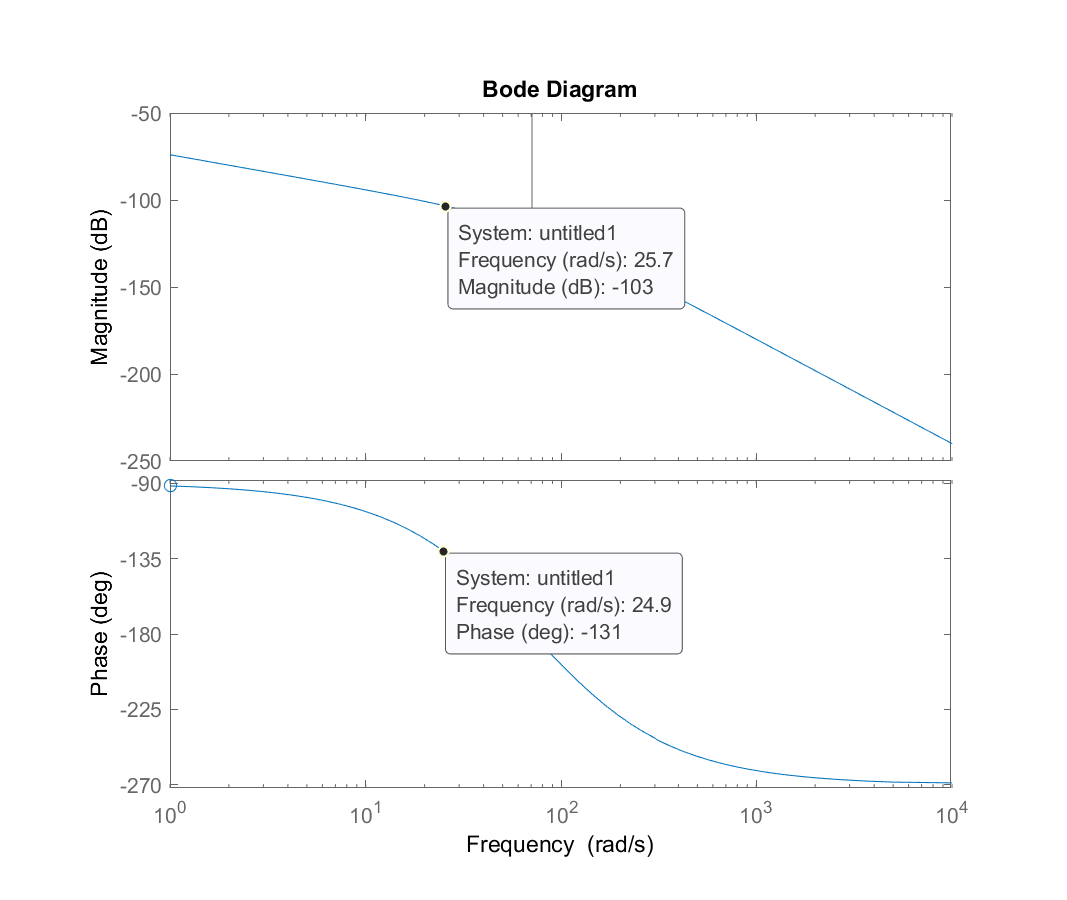
\includegraphics[width=0.65\linewidth]{bode_crossover.eps}
	\caption{Bodeho char. $L(s)$ na nové přechodové frekvenci}
	\label{fig:bode_crossover}
\end{figure}

Bodeho charakteristika pro otevřenou smyčku s tak silným regulátorem je na obrázku \ref{fig:bode_regulator}.
Po uzavření zpětné vazby získáme přenos $T(s) =\frac{L(s)}{1+L(s)}$, jehož odezva na jednotkový skok je na obrázku \ref{fig:step_response}.
Požadavky na návrh jsou zřejmě splněny, odezva uzavřené smyčky na jednotkový skok reference přestřelí pouze o 18.2\%, 
což je méně než požadovaných 20\%. Z tohoto důvodu stačí vzít i menší $K$, má volba však garantuje vyšší robustnost.

\begin{figure}[htbp]
    \centering % <-- added
\begin{subfigure}{0.48\textwidth}
  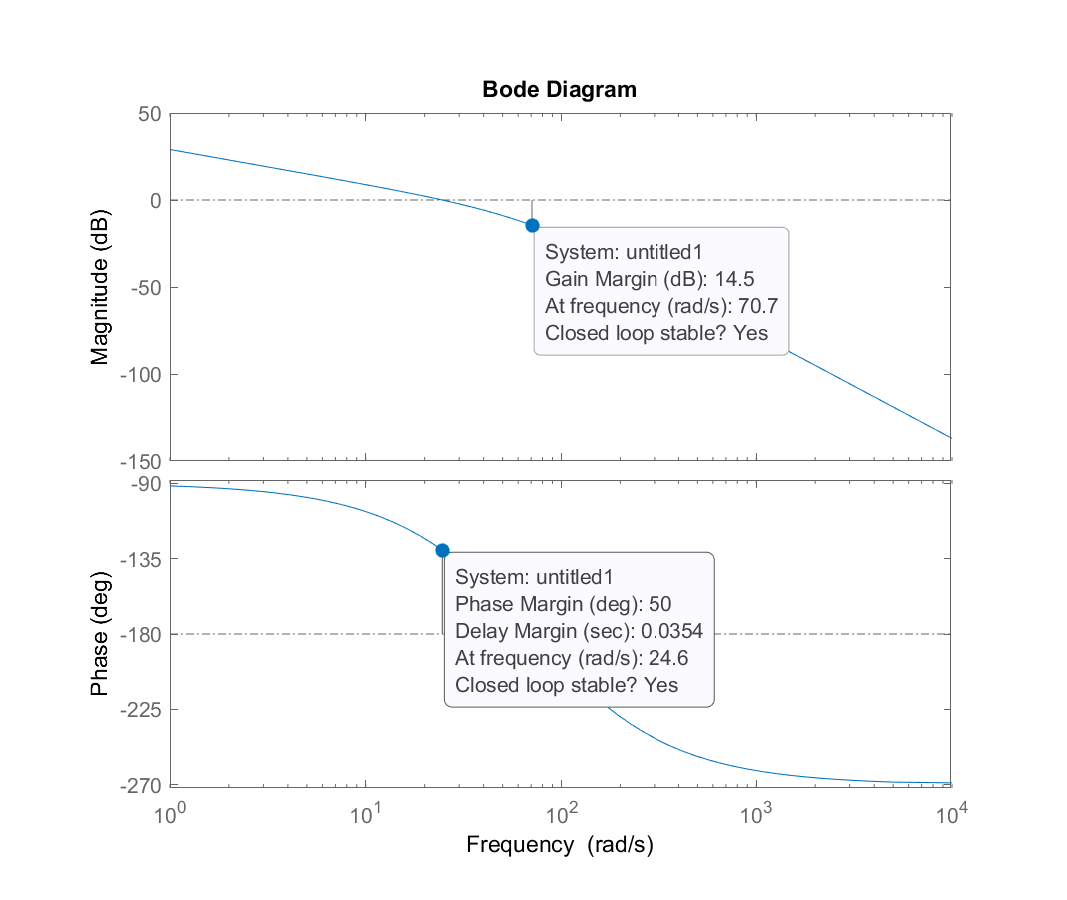
\includegraphics[width=\linewidth]{bode_novy.eps}
  \caption{Bodeho charakteristika $L(s)$ po přidání regulátoru}
  \label{fig:bode_regulator}
\end{subfigure}\hfil % <-- added
\begin{subfigure}{0.48\textwidth}
	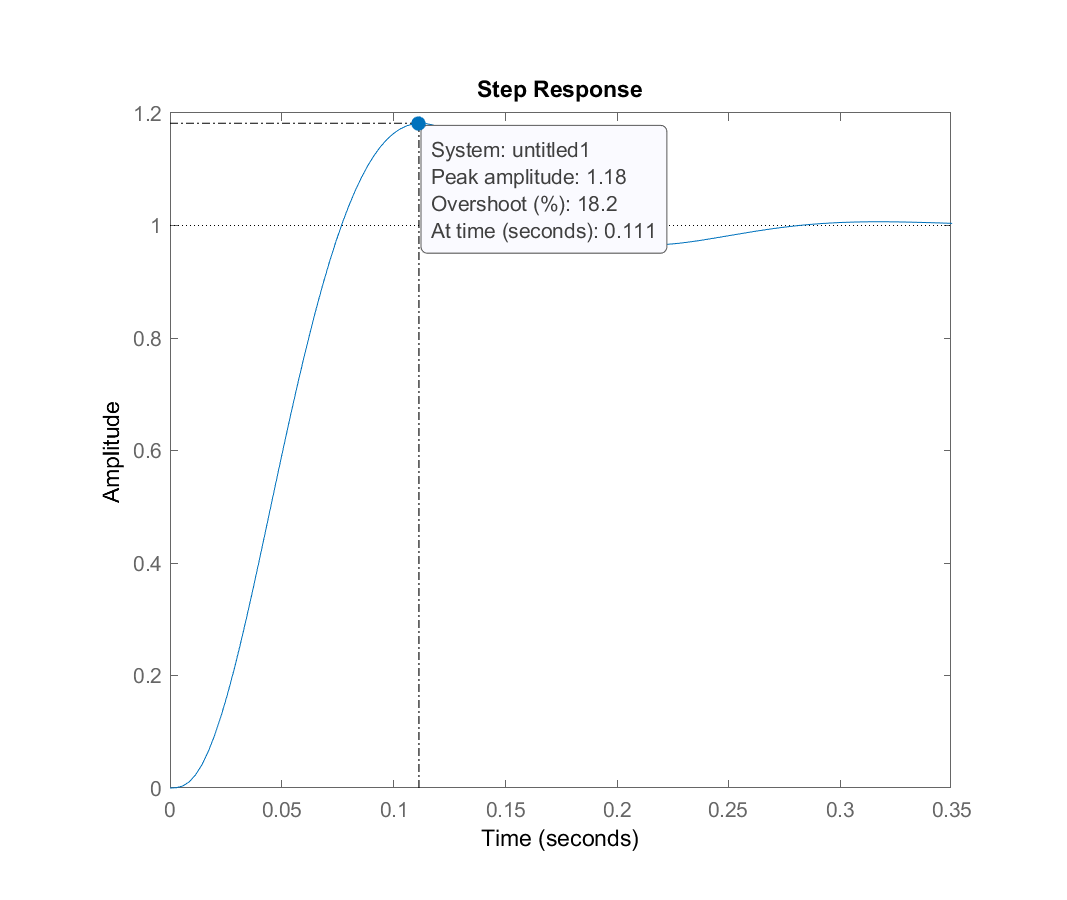
\includegraphics[width=\linewidth]{step_response.eps}
	\caption{Odezva uzavřené smyčky $T(s)$ na jednotkový skok reference}
	\label{fig:step_response}
\end{subfigure}
\end{figure}

\section{Charakteristiky ustáleného stavu v Bodeho grafu}
Jsem narozen 18. února, proto volím zadání za (b).
Na následujícím obrázku jsou frekvenční charakteristiky systému $L(j\omega)$. 
Pro vaše zadání z grafu určete \\
1) Typ systému, tj. řád astatismu \\
2) Konstanty ustáleného stavu $K_p$, $K_v$, $K_a$. \\
3) Ustálené odchylky na skok, rampu a parabolu referenčního signálu. \\
\textbf{Řešení:}

\begin{figure}[htbp]
	\centering
	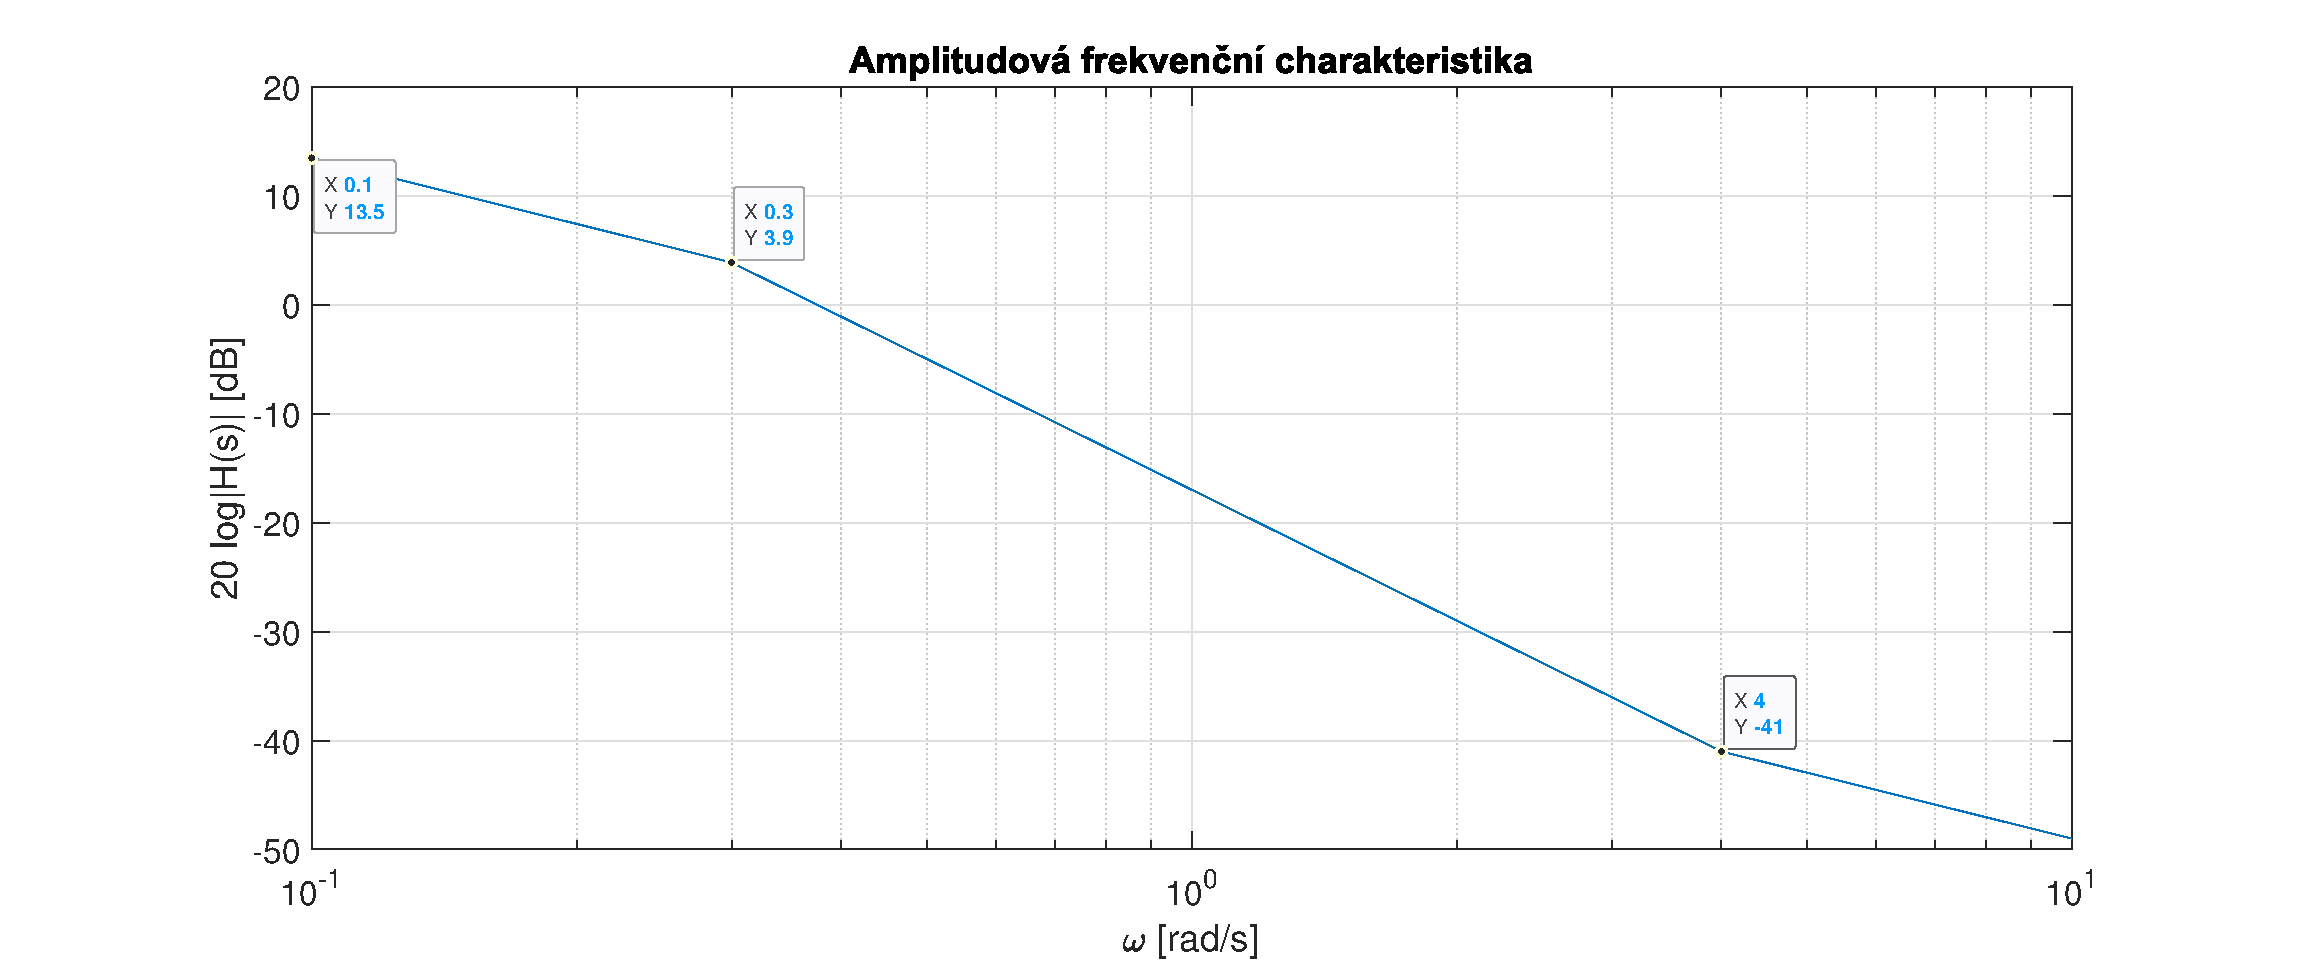
\includegraphics[width=\linewidth]{frek_zadani.eps}
	\caption{Zadaná frek. char. k vyšetření}
	\label{fig:frek_zadani}
\end{figure}

Nejdříve rekonstruuji zadanou frekvenční charakteristiku, protože v zadání jsou kóty velmi špatně čitelné. Nechť se přenos, jehož
amplitudovou frekvenční charakteristiku máme zadanou, jmenuje $H(s)$. Nejpřesněji identifikovatelná hodnota je $|H(0.5j)| = -5~\text{dB}$.
Zlomy charakteristiky nastávají na frekvencích 0.3 rad/s a 4 rad/s.
Se znalostí sklonů charakteristiky na jednotlivých uzavřených intervalech frekvencí lze dopočítat následující:
\begin{equation}
	\begin{split}
		|H(0.3j)| &= |H(0.5j)| - 40 \cdot \log(\frac{0.3}{0.5}) \approx 3.9 \text{dB} \\
		|H(0.1j)| &= |H(0.3j)| - 20 \cdot \log(\frac{0.1}{0.3}) = 13.5 \text{dB} \\
		|H(4j)| &= |H(0.3j)| - 40 \cdot \log(\frac{4}{0.3}) = -41 \text{dB} \\
		|H(10j)| &= |H(4j)| - 20 \cdot \log(\frac{10}{4}) = -49 \text{dB} \\
	\end{split}
\end{equation}
Podle těchto hodnot zrekonstruuji zadanou frekvenční charakteristiku na obrázku \ref{fig:frek_zadani}.

\subsection{Typ systému}
Typ systému lze identifikovat pohledem na nízké frekvence, protože
\begin{equation}
	\lim_{s \to 0} \underbrace{\frac{(s+z_1)(s+z_2)...}{s^l(s+p_1)(s+p_2)...}}_{=H(s)} = \frac{K_{\text{Bode}}}{s^l}.
\end{equation}
V mém zadání je pro nízké frekvence amplituda klesající se sklonem -20db/dekáda, proto je možné systém modelovat 
jako $\frac{K_{\text{Bode}}}{s^1}$ a pro $l = 1$ se jedná o systém typu 1 -- astatismus prvního řádu.

\subsection{Konstanty ustáleného stavu}
Konstanta polohy je vodorovnou asymptotou pro zesílení na nízkých frekvencích. Protože zadaná frek. char. přenosu $H(s)$
na nízkých frekvencích stále klesá, nachází se její vodorovná asymptota v $\infty$ dB. Proto $K_p = \infty$.

Konstanta rychlosti je číselně rovna frekvenci, na které asymptota pro $s \to 0$ protíná hladinu 0 dB.
Odečtením z obrázku \ref{fig:prolozeni_rychlost} lze určit přibližnou hodnotu $K_v \approx 0.45$.

Konstanta zrychlení by souvisela s asymptotou se sklonem -40dB/dekáda, ale tento sklon zadaná frekvenční charakteristika
pro $s \to 0$ vůbec nemá. Taková asymptota proto neexistuje a konstanta zrychlení je $K_a = 0$.
\begin{figure}[htbp]
	\centering
	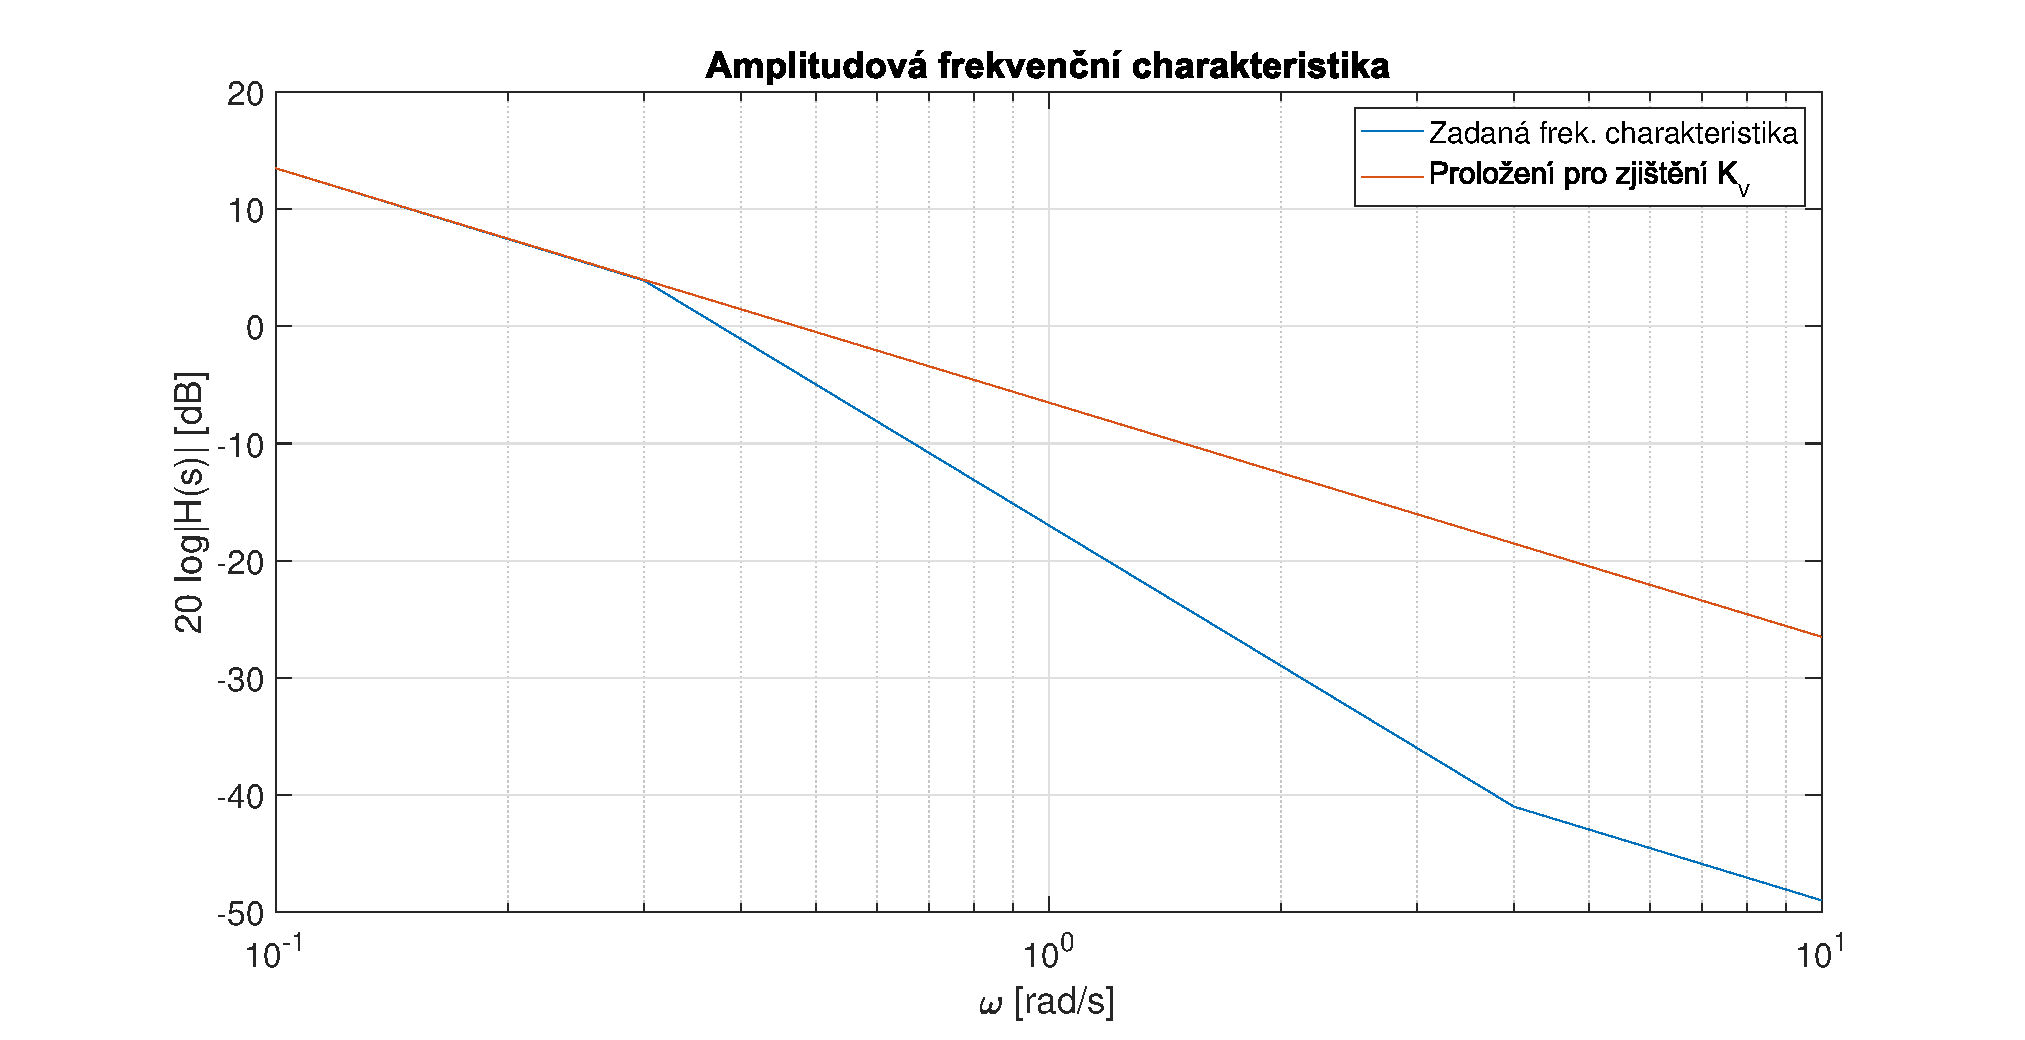
\includegraphics[width=\linewidth]{prolozeni_rychlost.eps}
	\caption{Frek. char. s proložením pro zjištění $K_v$}
	\label{fig:prolozeni_rychlost}
\end{figure}

\subsection{Ustálené odchylky}
Stačí dosadit do vztahů za dříve zjištěné hodnoty konstant polohy, rychlosti a zrychlení.
\begin{equation}
	\begin{split}
		e_{ss, step} &= \frac{1}{1+K_p} = 0\\
		e_{ss, rampa} &= \frac{1}{K_v} = \frac{20}{9}\\
		e_{ss, parabola} &= \frac{1}{K_a} = \infty
	\end{split}
\end{equation}
Všechny tři výsledky odpovídají očekávání. Zadaný systém vykazuje astatismus řádu jedna a proto je schopen
s nulovou odchylkou asymptoticky sledovat jednotkový skok, s nenulovou konečnou odchylkou sledovat rampu,
ale kvadratická funkce roste nade všechny meze a odchylka tak je nekonečná.

\begin{thebibliography}{9}

\bibitem{motivace}
	Robert H. Bishop, Supplementary lectures to book \emph{Modern control systems, 13th edition} 
		\url{https://www.youtube.com/watch?v=Wa_arqDWG3o}

\end{thebibliography}



\end{document}

